\section{Introduction}

A business rule articulates some aspect of the expected functional behavior (or a \textit{requirement})
of an enterprise application. Here is a simple business rule that determines how an invoice total is 
determined in a billing application:

\begin{quote}
	The \textit{Balance Type} of a customer affects how invoice total is computed; it can be 
	one of the following:

	\textit{None}: The customer's account will not hold a balance; instead all charges accrued 
	in an order will be included in the next invoice;
	
	\textit{Credit}: The customer's account may accrue charges up to the set credit limit. 
	Charges will automatically be paid from the users credit pool until the set limit is reached. 
	Users are responsible for paying their credit debt as well as any overages.
\end{quote}	

We will examine this rule closely later; for now, suffice it to say that the requirements 
of an enterprise system are typically captured by a large number (often in hundreds) of business rules
such as the one above.

It is reasonable to expect functional testing of an enterprise system to \textit{cover} its 
business rules, which is to say, testing would exercise every distinct scenario described in each of
its business rules.  For example, in the above rule, one of the scenario to be exercised is
that a customer's balance type is credit, and that the order amount does not exceed the customer's credit limit.
A test that exercises this scenario would set up a customer with the balance type as credit as well as a certain
credit limit, create an order with the appropriate constraint on the order total, and then finally
create an invoice for that customer, and verify the invoiced amount.  (See Figure~\ref{fig:jbilling-flow}.) 
Thus, it requires a carefully thought out test scenario (i.e. a sequence of test steps) as well as associated 
test data (i.e. values to be entered in the relevant test steps) to exercise a business rule, or a scenario 
thereof.

\begin{figure*}
\centering
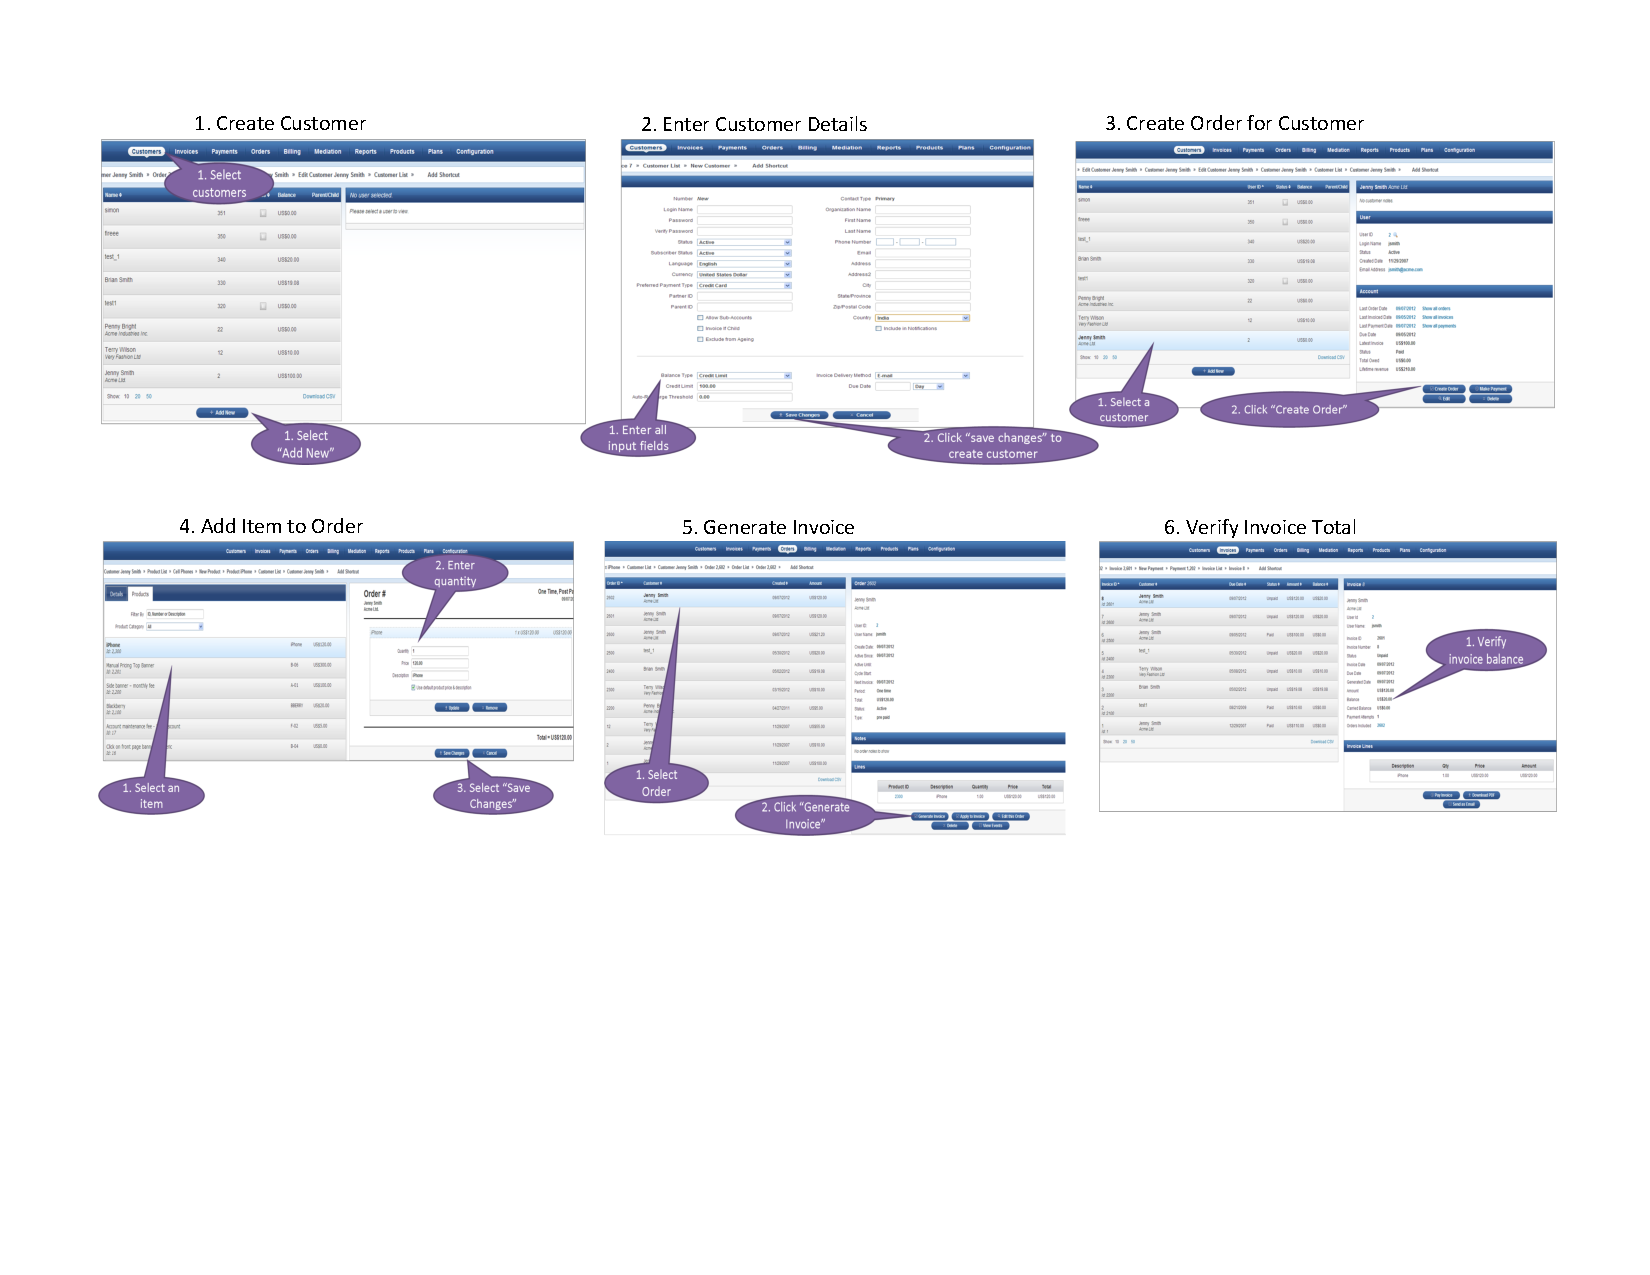
\includegraphics[trim=0 200 0 50,clip,width=7.5in]{figs/jbilling-flow}
\caption{Test sequence for a business rule from jBilling application}
\label{fig:jbilling-flow}
\end{figure*}

In practice, due to time pressures, testers are more often ad hoc than methodical in creating test 
scenarios and test data.  One part of the problem is that a realistic system might have hundreds of 
business rules written out in plain text, and it is difficult to grasp a global view of how the rules 
together describe the application behavior.  A related part of the problem is that it may need complex 
reasoning to piece together test sequences that would cover each scenario. Consequently, testers may end 
up creating a multitude of tests that exercise the same business rule, or a scenario thereof, over and over 
again without any additional benefit (especially if they are incentivised by the number of tests rather than 
quality), and more problematically, may neglect to create tests for some other business rules.  The net 
result is that despite a lot of resources spent in testing, bugs still escape into the field.

Our vision is to make testing of enterprise software more tool based, by adapting technology developed 
for automated and systematic test generation for programs.   In this vision, business rules would be 
written in a structured notation that allows mechanized analysis. 
(Special editors could be created to enable non-programmers to capture business rules in a structured notation; 
this is an independent challenge in \textit{end user} programming).  A tool would validate business rules 
and point out any ambiguities or omissions that it can detect.  After the business rules pass validation, 
another tool would generate test sequences and test data to exercise the application thoroughly as well as
without redundancies.

We have built a system to partially fulfil this vision.  In the rest of this introductory section, we
give an overview of our system, describe some of the challenges in automating test data generation, and 
briefly summarize our results.

%Randomly generated test data cannot be expected to suffice for enterprise
%applications with complex rules. Also, systematic test-generation approaches
%based on program analysis (\eg \cite{Emmi:2007,Li:2010,Marcozzi:2012,Pan:2011})
%cannot be expected to tackle enterprise applications, which use a mix of
%multiple language and database technologies in their implementation. Moreover,
%these techniques are directed toward attaining simple forms of code coverage,
%such as statement or branch coverage, rather than coverage of complex business
%rules.

\subsection{An overview}

Enterprise systems of interest to us are transaction oriented, which means that they consist of a set of
transactions or operations (e.g. create a customer, add an item to an order, and so on) that operate on databases.  
A business rule applies to a particular operation supported by the system.  Formally, a business rule
describes the relation between the database state before the operation and after it.  Figure~\ref{fig:invoice} shows
formalization of the business rule quoted informally at the beginning of the introduction.  It says that
the operation refers to an invoice record, \textit{inv}, and modifies specific attributes of \textit{inv}.
There are three scenarios that occur in this rule.  The first scenario applies when the customer to which the
invoice refers has balance type \textit{None}; the \textit{precondition} is shown on the left of the first arrow.  
Note that the invoice has references to the customer to which this invoice pertains, 
as well as an order created in the system; in a relational database, these would be foreign keys in customer and 
order table.  The second scenario applies when the customer has balance type \textit{credit}, but the credit limit 
is sufficient to cover the order total.    The third scenario applies when the customer has balance type 
\textit{credit}, but the order total exceeds the credit limit.  In each scenario, the effect of the operation is to 
compute invoice total, and update the customer's residual credit limit; this effect, or \textit{postcondition} is 
shown to the right of the arrow in each case.  Note that business rules refer to state observable at transaction 
boundaries; intermediate program states encountered in the implementation while a transaction is in process, are 
not important to business rules.

\begin{figure}
\centering
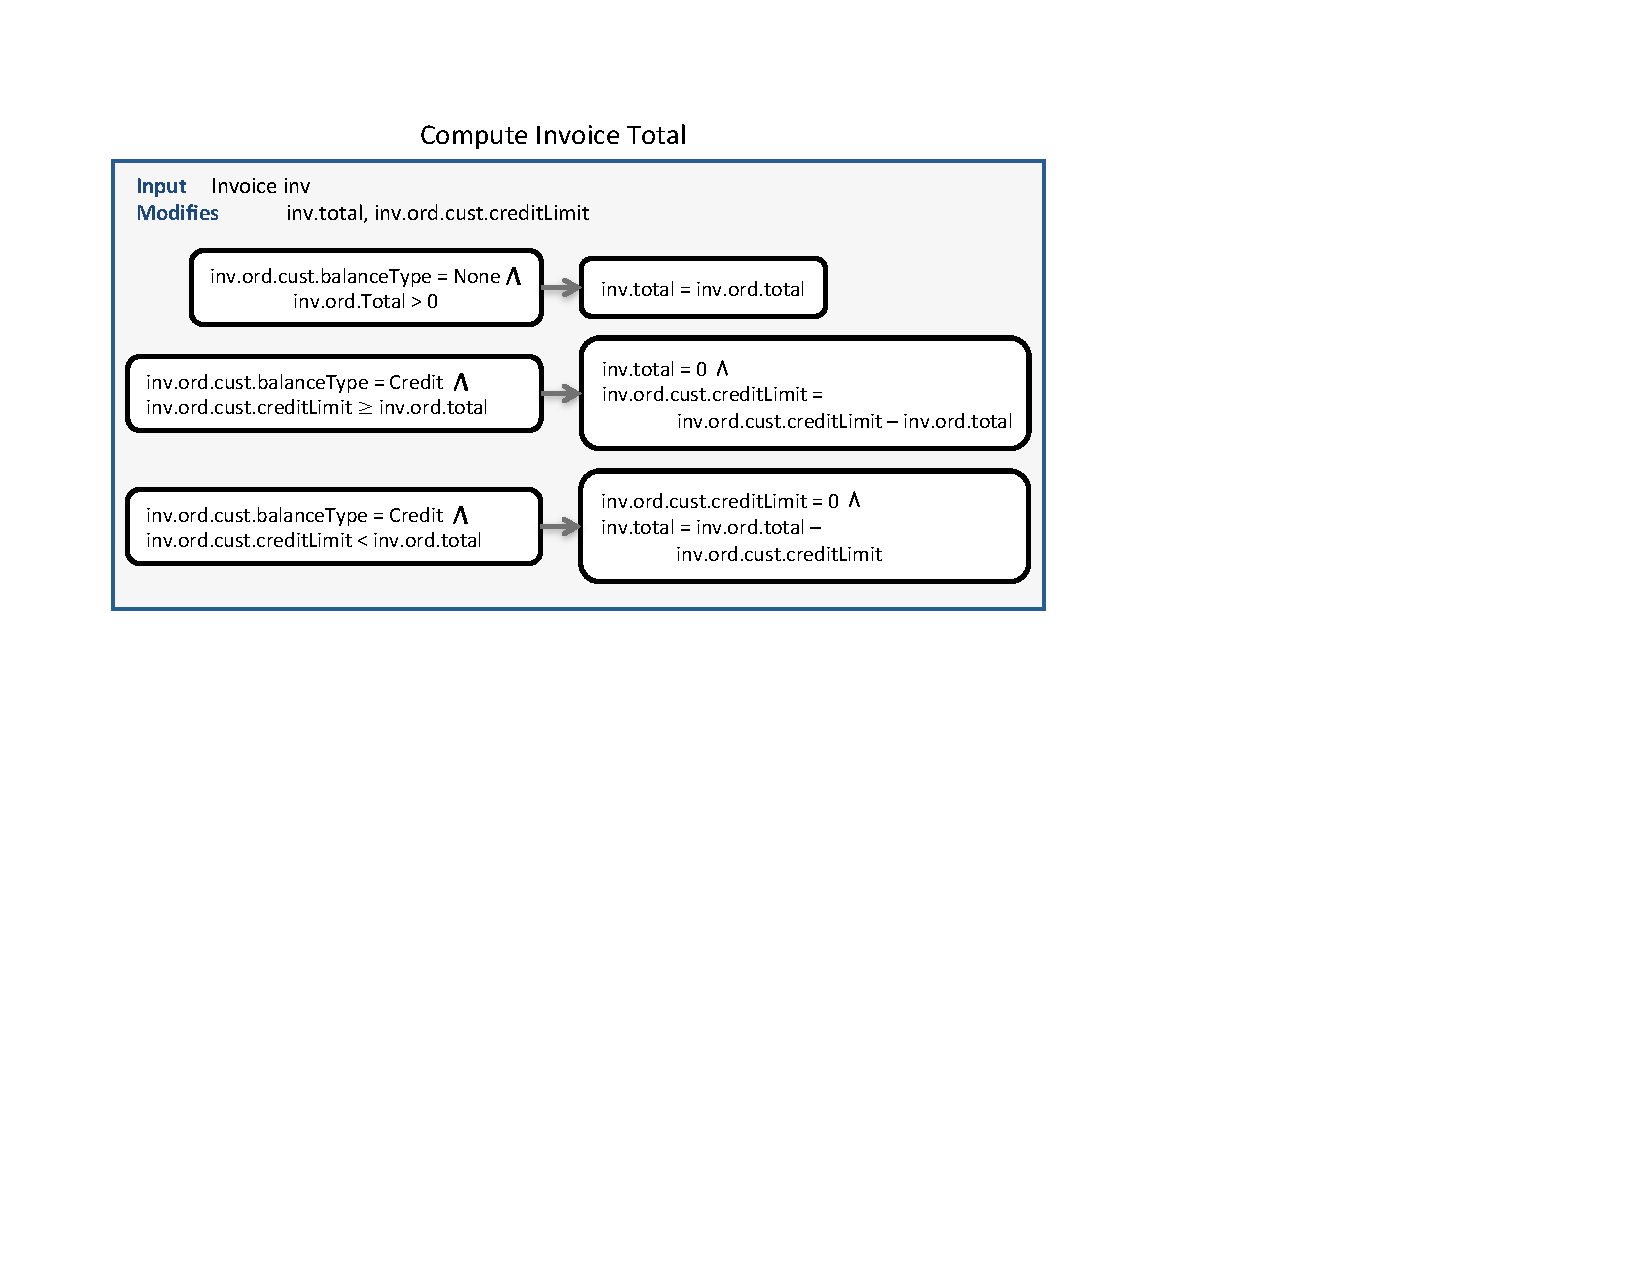
\includegraphics[trim=30 300 270 0,clip,width=\columnwidth]{figs/invoice}
\caption{Business rule for computing invoice amount}
\label{fig:invoice}
\end{figure}

Coering a business rule means to exercise each of its constituent scenarios, referred henceforth as \textit{ruleparts}.
To cover these three ruleparts in the business rule of Figure~\ref{fig:invoice}, it is necessary to create (separate)
each of the three preconditions, and in each case verify that the post condition holds after the operation has completed.  
This brings us to the main difficulty in creating tests:  appropriate database state, such as a customer with a certain 
balance type, and an order with a certain amount, needs to be established before any of these scenarios can be exercised.  
We showed in Figure~\ref{fig:jbilling-flow} the steps that would be required to create these preconditions 
(applicable to each of the three scenarios, though the test data would need to be different).   How can we
identify these steps, and the data to be entered in each of these steps automatically to cover a rulepart of
a business rule?

Our observation is that the steps that are required to drive the database state to a desired precondition are
carried out by operations, and those operations too would have rules that specify their functionality.  We could
then use business rules as ``state transformers'' and piece together a sequence of operations to arrive at
a desired state.  The advantage of looking at business rules as state transformers is that we can adapt the
technology developed for test generation on \textit{programs} for the problem at hand.  We clarify and emphasize, 
though, that business rules are themselves not executable programs; rather they only are an abstract description 
of the functionality of a program.

At a high level, the idea is to use backward analysis to piece together a sequence of operations to arrive at 
a desired state.  We look for an operation whose business rule has a rulepart whose postcondition would imply the 
desired precondition.  Such an operation, if executed in a way that that specific rulepart applies, would establish 
the desired state.  The operation may require some user-provided values, but may partially rely on prior database
state. The process is repeated until no prior database state is assumed, that is, all the database state is 
established by operations identified in the process.  

Consider the second rulepart of the rule showed in Figure~\ref{fig:invoice}. The operation here is to generate
an invoice.  But  


The idea of backward traversal is definitely not novel; it is reminiscent of weakest preconditions.  Our
contribution is to make this idea work in the context of business rules.  We solved several engineering 
challenges ...


\subsection{Related work}

TODO move to another section.

At first blush, this problem seems to be reminiscent of the problem of generating tests for programs 
written as control-flow graphs, with the goal of exercising each acyclic path in the program, if
possible.  There have been a number of techniques in the literature for test generation. Mostly
notably, techniques such as \textit{concolic} testing attempt to identify a series of test data 
that would force program execution thorough different paths.  Other approaches are based on model
checking, with the goal of creating test inputs to reach specific program states.

However, the problem of test generation from business rules is different.  Business rules do not
describe the implementation of a system: rather they only describe a model.  (Model-based test 
generation?)
